\chapter{State Of The Art}
This chapter describes the main working instrument used for this work: the cognitive architecture \emph{\mbox{ACT-R}} and the computer vision library \emph{\mbox{OpenCV}}. 

%TODO inserire in act-r
  %% Cognitive Architecture
\begin{comment}
 \section{Cognitive Architecture}	
	A cognitive architecture is the implementation through computer simulation softwares \todo{controllare correttezza di softwares} of a theory about human cognition. The theory generally relies on a wide selection of human experimental data. The design of these architectures tries to simulate human intelligence in a humanlike way.
	
	
	
	As the term \emph{infrastructure} suggests, cognitive architectures usually are built aggregating many software modules, most of which represent functions of the human brain. Anyway, there exist other modules, which coordinate the overall functioning and without which the whole architecture could not work. In the following section, which describes \emph{ACT-R}, the \emph{procedural module} is an example of such modules. In fact, it does not represent a function of the human being, though it is necessary to coordinate the communication between all the other modules. 
	
	Some architectures, can, in addition, include some \emph{learning mechanisms}. This can be the attempt to simulate the human memory system, thanks to which the behaviour of a human can be different after having experienced facts or consequences of a specific choice ~\cite{Sears2012}.
\end{comment}
	
	
  %% ACT-R
  \section{ACT-R}
	\mbox{ACT-R}, that stands for \emph{Adaptive Control of Thought-Rational}, is a cognitive architecture, i.e. a computer implementation of a theory about human cognition. As such, it models the structure and behavior of the human brain trying to explain how all the components of the brain work together and form the human mind.

	The following sections describe the theory on which ACT-R relies, how the theory is implemented in the framework and the concept of \emph{model}.  

\begin{comment}
	 
	\mbox{ACT-R} is a software written in Lisp and its models are written in a Lisp-like language. It is thought to have a modular structure so that it can be easily extended. The current version of the software is the 6.0. 

	
\end{comment}	

	
	
	\subsection{The Theory Behind ACT-R}
		The following section describes two fundamental assumptions on which ACT-R relies, the \emph{Unified Theory About Cognition} and the classification of the human memory in \emph{declarative} and \emph{procedural}. Both of these assumptions are important because they determinate the structure of the framework.
		
		\subsubsection{Unified Theory About Cognition}
		\mbox{ACT-R} implements the homonym theory developed by John Robert Anderson, professor of psychology and computer science at Carnegie Mellon University. Such theory tries to explain the overall behavior of the human mind through connections between its well-defined components that, combined together, form an integrated system. The following quote, that explains the meaning of integrated system, comes from Allen Newell, the man who inspired Anderson in creating ACT-R theory~\cite{Anderson04anintegrated}.

		\begin{quote}
		A single system (mind) produces all aspects of behavior. It is one mind that minds them all. Even if the mind has parts, modules, components, or whatever, they all mesh together to produce behavior. Any bit of behavior has causal tendrils that extend back through large parts of the total cognitive system before grounding in the environmental situation of some earlier times. If a theory covers only one part or component, it flirts with trouble from the start. It goes without saying that there are dissociations, independencies, impenetrabilities, and modularities. These all help to break the web of each bit of behavior being shaped by an unlimited set of antecedents. So they are important to understand and help to make that theory simple enough to use. But they don’t remove the necessity of a theory that provides the total picture and explains the role of the parts and why they exist~\cite[p.17-18]{newell1994unified}.
		\end{quote}

  

		\subsubsection{Declarative memory and procedural memory}
		In psychology, \emph{memory} is defined as the processes by which information is encoded, stored and retrieved ~\cite{baddeley2009memory}. 
	
		\mbox{ACT-R's} most important assumption about knowledge is based on Anderson's theory about memory. 
		Anderson divides memory into \emph{declarative} and \emph{procedural}~\cite{Anderson04anintegrated}. 
	
		Declarative memory refers to all the information that can be consciously recalled. This kind of knowledge comprehends facts and notions that human beings explicitly know. To call back this kind of information, there must be a conscious process by the human being. For this reason, this kind of memory is also called \emph{explicit}.
	
		In contrast, procedural memory refers to all that notions or skills that human beings have but which they learnt in an implicit way. Examples of this knowledge are driving, reading and writing. In this case, in order to call back this kind of information, the human being does not need a conscious process. That is why this kind of memory is also called \emph{implicit}~\cite{anderson1976language}. 
			
		When a person starts learning typewriting, for example, an attempt he can make in the beginning is trying to memorize the layout of the keyboard. The aware knowledge of all the positions of the keys is the declarative memory. After having become a skilled typewriter, the same person will type faster putting his fingers on the right keys and pushing them in the correct order, without thinking anymore about the positions of the keys on the keyboard. Moreover, if someone asks him where the position of a certain character is on the keyboard, he will probably answer that he can not say it without looking at it. This is because, now, for this task he is using his procedural memory~\cite{anderson1993rules}.
	
	\subsection{The Architecture}
		 This section, after having defined \emph{chunks} and \emph{productions}, the building blocks of ACT-R structure, presents the architecture of the framework.

		\subsubsection{Chunks and productions}
		In \mbox{ACT-R}, declarative memory is represented by structures, called \emph{chunks}, and procedural memory  by rules, called \emph{productions}. Chunks and productions are the basic building blocks of ACT-R \emph{models}. The concept of model will be described in \ref{modelSect}.
	
		The \emph{chunks} are data structures which are defined by their \emph{type} and their \emph{attribute list}. This is a tuple of pairs, each of which is made up by a fixed part and a variable part.
		The fixed part is the \emph{name} of the attribute and is called \emph{slot}.
		The variable part is the \emph{value} of the attribute.
		Each chunk has also a \emph{name} but it is not considered to be a part of the chunk itself, as it does not exist in \mbox{ACT-R} theory. It is used only for convenience to reference the specific chunk when writing models. The chunk-types can be organized into hierarchies.
	
		The \emph{productions} are \mbox{ACT-R} equivalent of functions. They define sequences of actions and can be fired only if a set of preconditions is satisfied. They can be represented as \emph{if-then} rules, where the \emph{if-part} is a set of conditions that must be true for the production to apply and the \emph{then-part} is the action of the production and consists of the operations the model should perform when the production is selected and used. 

		In general there could be some conflicts between productions. This happens when preconditions of two or more productions are satisfied at the same time. In these cases the production to be fired is the one with the highest \emph{utility value}, a numeric quantity which gives a priority measure. It can be set a priori by the modeler or learnt while the model is running. The latter, together with the fact that in the calculation of this value the probability of reaching the goal and the time estimate are included, constitutes the basis of the learning mechanism embedded in \mbox{ACT-R}: the more successfully a production is, the more its estimated probability and utility grow, increasing the probability for that production to be selected again~\cite{actr6refman}.
	

		\subsubsection{Organization of the Modules}
		All the activities carried out by the human brain, like talking or moving, are performed by neurons located close together in a well defined and limited area of the cortex. Trying to imitate this "architecture", \mbox{ACT-R's} framework is structured in different \emph{modules}, each of which represents one specific function of the human brain. 
	
		Figure \ref{fig:modulesActr} shows the modular structure of ACT-R. In the picture you can see two groups of modules, separated by the \emph{procedural module}. 
	
		The first group comprehends \emph{visual}, \emph{aural}, \emph{manual } and \emph{vocal modules}. These let the model interact with the environment.
		The \emph{visual module} is responsible for recognizing objects in the visual scene and shifting the focus to them. Similarly, the \emph{aural module} identifies sounds and moves the attention to them. 
		The \emph{manual module} can move the virtual hands and perform actions like pressing the key on a keyboard or moving the mouse while the \emph{vocal module} controls the virtual voice.
	
		The other group comprehends \emph{goal module}, \emph{imaginal module} and \emph{declarative module}. These represent the internal information of the model.  
		The \emph{goal module} provides the system with the structure of the goal of the task, defined as a chunk. 
		The \emph{imaginal module} has to contain and update the current context relevant to the current task. 
		The \emph{declarative module} provides the model with a declarative memory, thus it stores the declarative chunks generated by the model and provides a mechanism for retrieving them. 
	
		Finally, the \emph{procedural module} is responsible of the communication and the coordination of all the other modules. 
	
		\begin{figure}[h]
		  \begin{center} 
		    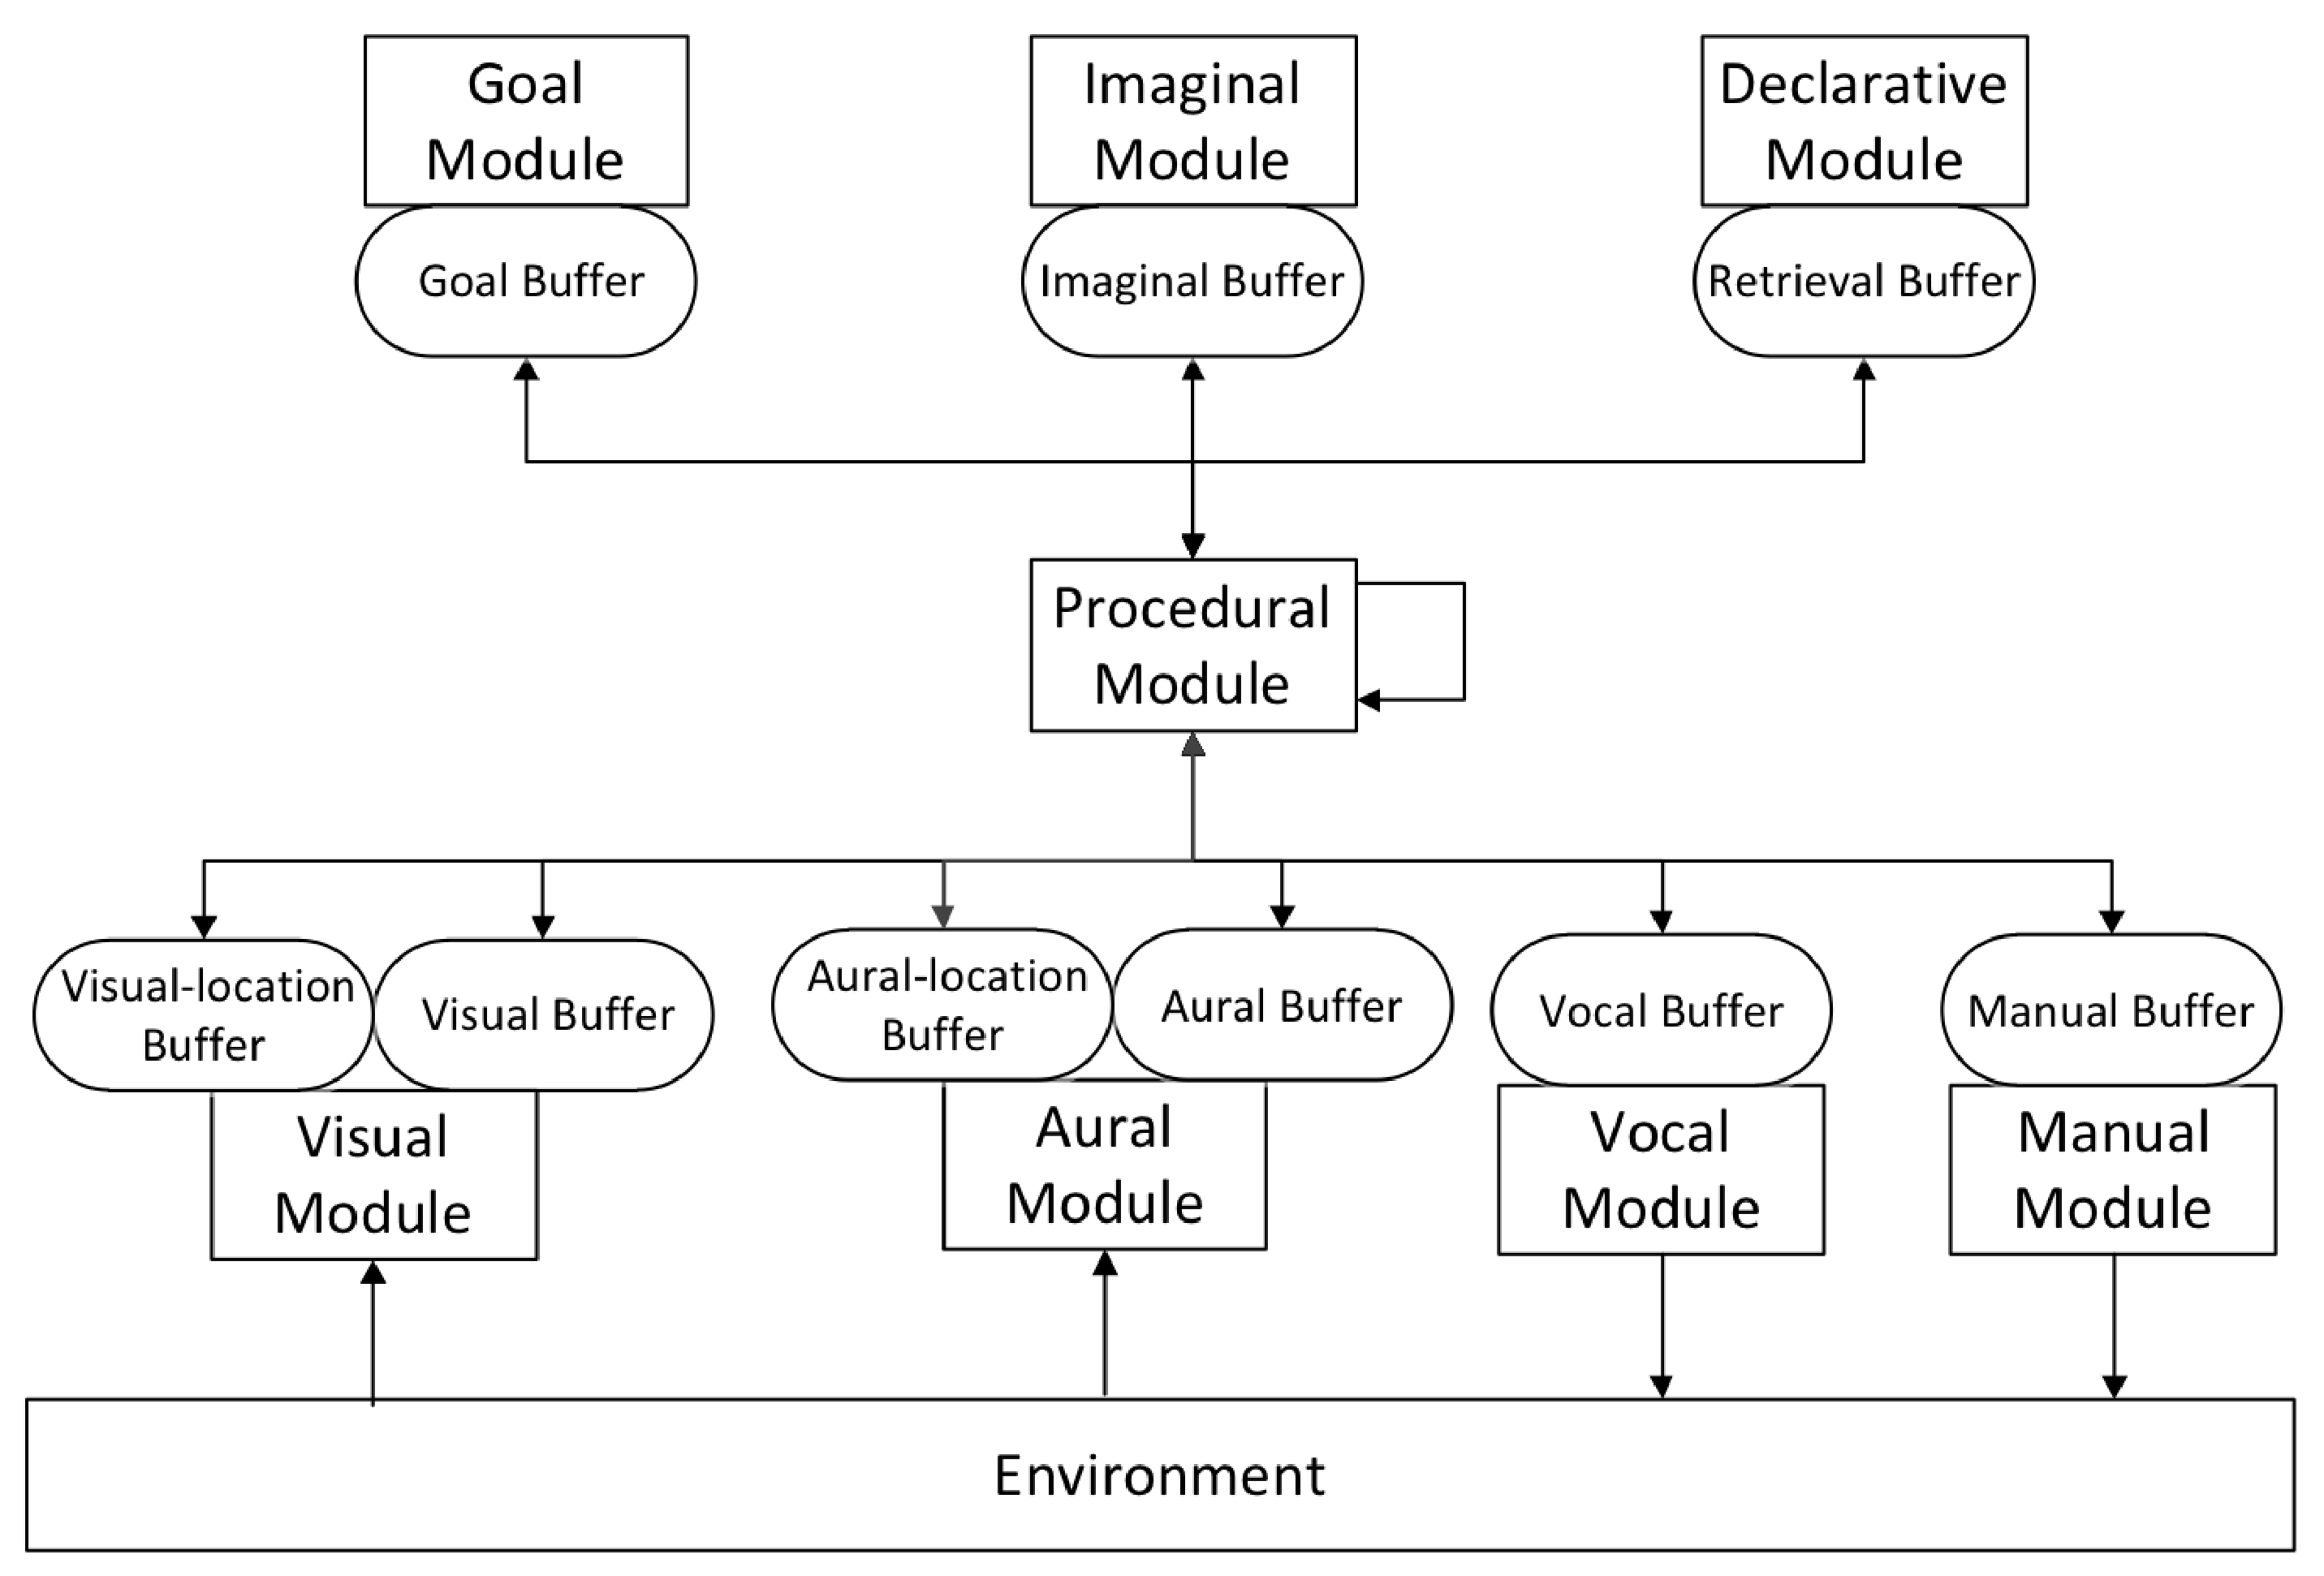
\includegraphics[scale=0.25]{images/ch_01/actr.eps}
		  \end{center} 
		  \caption{\textit{Structure of ACT-R.}}  
		  \label{fig:modulesActr}
		\end{figure}
	
	
		All the modules are independent of each other, they do not share variables or information. They can communicate with each other through \emph{buffers}, which represent the interface of a module towards the others. A module can have no buffers as well as one or more than one. The communication consists in exchanging chunks. Each module can read chunks from every buffer but it can make changes only to the chunks in its own buffers. Moreover each buffer can hold one chunk at a time. 

		Although modules usually work in a parallel way, their interactions can be only serial.
		There are two reasons for this limitation: the first one is that the structure of the buffers can hold only one chunk at a time and the second one is that only one production can be fired at a time~\cite{actr6refman}.
	
	\subsection{ACT-R Models}\label{modelSect}
	ACT-R is able to perform several task-independent reasoning. 
	To adapt these reasoning to a single task it is necessary an additional layer called \emph{model}.

	Each model contains the specific modelers' assumptions about the task within ACT-R view of cognition. That knowledge is expressed through productions that, when the model is running, interact with the modules, querying them and reading their buffers. 
	
	Running a model produces a series of atomic cognitive operations which step-by-step leads to the solution of the task. Each operation is associated with quantitative and qualitative measures like the correctness of the goal and the time necessary to complete the operation.
	This fact gives the model the possibility to predict the sequence of cognitive actions produced by human beings when they try to solve the same task.
	Comparisons with human performances can be useful to evaluate the quality of the models~\cite{Sears2012}.

	ACT-R is written in Lisp and provides its own lisp-like language for the modelers to write the models.



		

	%TODO allungare (di parecchio)	questa parte
  %% OPENCV
  \section{OpenCV}
	\mbox{OpenCV}, an abbreviation that stands for \emph{Open Source Computer Vision}, is a computer vision library that was originally developed by Intel and, later on, by Willow Garage.
	It is a cross-platform library and can run under Linux, Windows and Mac OS X. 
	It is released under a BSD license, thus it is free and open source. 
	In the beginning it was developed in C and C++ and afterwards it was expanded by the addition of interfaces for other languages as, for example, Java, Python, Ruby and Matlab. 

	\mbox{OpenCV} is designed for computational efficiency and with a strong focus on real-time applications. On Intel architectures there is the possibility to further optimize the library thanks to Intel's \emph{IPP} library. IPP library, that stands for \emph{Integrated Performance Primitives}, contains a series of low-level optimized routines in many different algorithmic areas. If this library is installed, \mbox{OpenCV} uses it automatically at runtime.

	\mbox{OpenCV} offers a simple to use infrastructure that helps programmers create quite complicated vision applications in an acceptable time. The version 2.4 has more than 2500 algorithms that cover many areas of vision. The library has been used in many applications as, for example, mine inspection and robotics. 
	It also contains \emph{MLL}, a full and general purpose \emph{Machine Learning Library}, which provides functions for pattern recognition and clustering~\cite{bradski2008learning,OpenCV:MainWebPage}. 

	The following sections contain an introduction to computer vision, a brief history of OpenCV library, a description of its main features and an overview of its architecture. 
	%The aim of this work is not to list and describe all the algorithms and techniques implemented in the computer vision library. 
	For more information about computer vision see texts by Trucco~\cite{trucco1998introductory} for a simple introduction, Forsyth~\cite{forsyth2011computer} as a comprehensive reference, and Hartley~\cite{hartley2003multiple} and Faugeras~\cite{faugeras1993three} for how 3D vision really works.

	
	\subsection{Introduction to Computer Vision}
	Computer vision is the transformation of image or video data into a new representation. Such representation can be either another image, for example a gray-scale version of the original one, or even a decision based on the information extracted from the input data. 
	Often computer vision algorithms use contextual information in order to simplify the problem.

	People not expert in computer vision may mislead the complexity of its tasks. Often, in fact, even a very simple operation for the human brain, like recognizing an animal in a picture, represents a very complex task for a machine. 
	Human visual system is very complex. It divides the visual signals into many channels, each of which brings a different kind of information to the brain. The brain uses an attention system which identifies important parts of the image and focuses on them, excluding the analysis of the remaining parts. Moreover, further information coming from all the other senses and the experience acquired during the whole life of the person completes the analysis of the image, in a way still not completely understood. All these factors create the visual perception of human beings.

	In a machine vision system, instead, when the computer receives an image or a video from a camera, it receives simply a grid of numbers. In most of cases, there are no mechanisms for pattern recognition, automatic control of aperture and focus of the camera nor cross-associations with other senses or experience.  
	Figure \ref{fig:imgMatrix} explains this concept. The machine does not recognize automatically the side mirror of the car, it sees just a grid of numbers. A goal of computer vision is to turn the grid that describes this particular object into the object itself. 
	
	
	\begin{figure}[h]
	  \begin{center} 
	    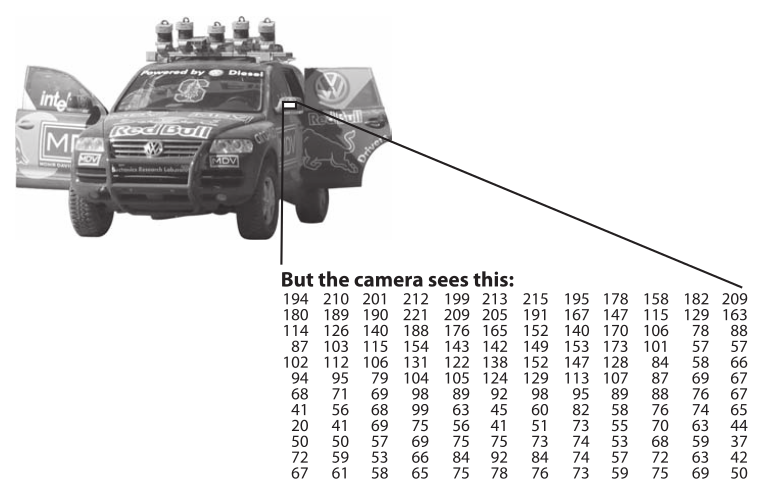
\includegraphics[scale=0.6]{images/ch_01/img_matrix.png}
	  \end{center} 
	  \caption{\textit{Representation of an image in a computer vision system.}}  
	  \label{fig:imgMatrix}
	\end{figure}

	Figure \ref{fig:2d3d} shows another aspect that makes computer vision tasks so difficult to solve. An image is a 2D description of a 3D world. The problem in the way it is posed is impossible to solve. There are infinite possible ways to reconstruct a 3D world from a 2D image. As shown in the picture, the solution changes with the point of view of the camera. This is formally an ill-posed problem.

	\begin{figure}[h]
	  \begin{center} 
	    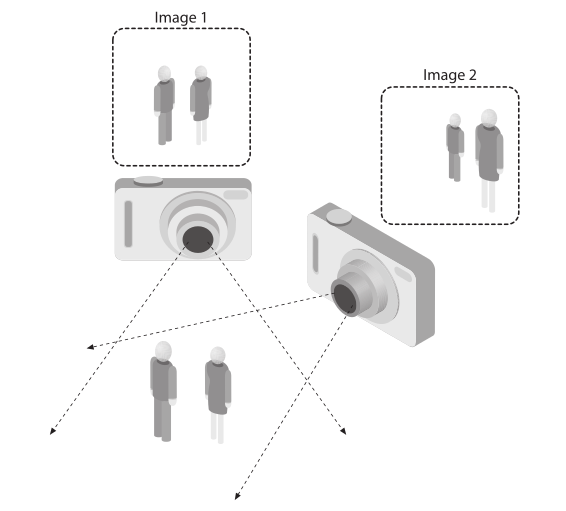
\includegraphics[scale=0.6]{images/ch_01/2d_3d.png}
	  \end{center} 
	  \caption{\textit{How the 2d representation changes with the viewpoint}}  
	  \label{fig:2d3d}
	\end{figure}

	Moreover, generally speaking, data is affected by noise. The word noise comprehends all the possible variations in the world, like weather, lightning, reflections and movements, and all the imperfections affecting the input mechanisms, like errors of the lens or of the sensors. 
	
	Some causes of noise are easy to remove. The errors caused by the lens, for example, can be mathematically described by polynomial functions, thus it is quite simple to correct them. 
	The environment variations, instead, are not well known a priori, hence are more difficult to delete. Typically, this category of noise is dealt with statistical methods, that generally do not remove it completely but attenuate it. Say, for example, to have many different pictures of the same visual scene, every one taken in different conditions of weather, lightning, reflections and so on. In this case the noise is considered, statistically speaking, a white noise. A statistical approach suggests to make the average of all the pictures. In this way, the features of the image remain, while the noise is reduced by the average operation.
	
	A common way to simplify the problem of computer vision is to add contextual knowledge to the solution. 
	Consider the example of a mobile robot which has to find and pick up staplers in a building. The robot can use the fact that the staplers are always on desks. This fact gives the robot an implicit information about the size and the position of the object, that brings it to exclude false "recognitions". Moreover, if all the desks have rectangular shapes, are made of wood and have the same color, the computer vision system can use this additional information to exclude other false staplers, increasing the accuracy of the research. As general rule: \emph{"the more constrained a computer vision context is, the more we can rely on those constraints to simplify the problem and the more reliable our final solution will be"}~\cite[5]{bradski2008learning}. Of course, in this way, the solution is not general purpose any more.
	
	Machine learning techniques allow to extract variables that model contextual information from a limited number of training cases and using them to solve other instances of the modeled problem. 
	Differently from the previous example, such variables are not set a priory by the modeler but are learnt from a series of trials. For this reason they can be hidden parameters or may even not represent physical quantities and remain mathematical variables~\cite{bradski2008learning}.

	\subsection{OpenCV History}
	The \mbox{OpenCV} Project starts in 1999 as an Intel Research initiative aimed to improve CPU intensive applications as a part of projects including real-time ray tracing, which in computer graphics is a particular technique for generating images, and 3D display walls. The early goals of the project are: developing optimized code for basic vision infrastructure, spreading this infrastructure to developers and making it portable and available for free, using a license that allows the developers to create both commercial and free applications.

	The first alpha version is released to the public in 2000, followed by five beta versions between 2001 and 2005, which lead to version 1.0 in 2006. In 2008, the technology incubator Willow Garage begins supporting the project and, in the same year, version 1.1  is released.

	In October 2009, \mbox{OpenCV} 2.0 is released. It includes many improvements, such as a better C++ interface, more programming patterns, new functions and an optimization for multi-core architectures. According to the current \mbox{OpenCV} release plan, a new version of the library is delivered on a six-months basis. \cite{OpenCV:ChangeLogs}.



	\subsection{Main Features}
	\mbox{OpenCV} offers a wide range of possibilities. First of all, it provides an easy way to manage image and video data types. It also offers functions to load, copy, edit, convert and store images and a basic graphical user interface that allows the developers to handle keyboard and mouse and display images and videos. The library permits to manipulate images even with matrix and vector algebra routines. It supports the most common dynamic data structures and offers many different basic image processing functions: filtering, edge and corner detection, color conversion, sampling and interpolation, morphological operations, histograms and image pyramids. Beyond this, it integrates many functions for structural analysis of the image, camera calibration, motion analysis, object recognition and machine learning. \cite{Agam2006}.

	%\todo{espandere (dopo aver scritto la parte di architettura)}
	
	\subsection{Architecture}
	Since version 2.2, the \mbox{OpenCV} library is divided into several modules, built in library files. Each module serves a specific purpose and includes functions in order to accomplish it. 
\begin{comment}	
The modules are:
	\begin{itemize}
	    		\item the \emph{core module}, that contains the core functionalities of the library, i.e. the basic data structures and functions used by all the other modules. The functions 
			\item ;
			\item ;
			\item .
	\end{itemize}
\end{comment}

	The \emph{core module} contains the core functionalities of the library, i.e. the basic data structures, both in C and \mbox{C++} languages, and a variety of functions used by all the other modules. Such functions have many purposes: operating on arrays and matrices, drawing shapes on the images, storing and restoring library data structures and primitive data types in \mbox{XML} and \mbox{YAML} formats and other.
	
	The \emph{imgproc module} contains the main image processing functions. Processing an image means \emph{"using higher-level operators that are defined on image structures in order to accomplish tasks whose meaning is naturally defined in the context of graphical, visual images"}~\cite[128]{bradski2008learning}.
	Such functions are, for example, operations to perform various linear or non-linear filtering on 2D images, geometrical transformations of 2D images (resize, affine and perspective warping, generic table-based remapping), color space conversions, histogram analysis, feature detection and object detection.
	
	The \emph{highgui module} allows the library to interact with the operating system, the file system and hardware such as cameras. Its interface permits to open windows, display images, read and write graphics-related files, both images and video, and handle simple mouse, pointer, and keyboard events. It also allows to add simple user interface elements to the displayed windows.   

	The \emph{features2d module} allows to use different algorithms to implement the \emph{interest points processing}. This technique relies on the idea that instead of analyzing the complete image it is better to work on a limited number of particular pixels. Such points must be distinguishable features in all the images in which they must be detected. 
	To do this, the module offers functions for feature detection, feature description and descriptor matching.

	The \emph{calib3d module} focuses on camera calibration and stereo vision. Camera calibration permits to modify images and videos by correcting the errors derived by the use of lenses. Stereo vision allows to have benefits from all the advantages given by using two equal cameras instead of one, like for example measuring distances with high precision.

	The \emph{video module} implements some techniques for video processing, in particular \emph{motion estimation}, \emph{feature tracking}, and \emph{foreground extraction} algorithms. Motion estimation techniques define motion vectors that describe the transformation from consequent frames. Feature tracking algorithms improve motion estimation by working only with some features instead of sets of pixels. Foreground extraction algorithms try to recognize foreground objects of interest comparing an observed image with an estimate of the same image as if it contained no objects of interest. 

	 The \emph{objdetect module} allows the detection of particular categories of objects such as faces or cars. To do so, it uses functions for training the software in recognizing a particular class of objects and verifying if an input image contains such kind of object once the learning is terminated. 

	\mbox{OpenCV} also includes other utility modules: the \emph{ml module} contains machine learning functions, the \emph{flann module} computational geometry algorithms, the \emph{contrib module} some contributed code, the \emph{legacy module} some obsolete code and the \emph{gpu module} support for gpu acceleration ~\cite{laganiere2011opencv,OpenCVDoc,bradski2008learning}.


